\documentclass[times, utf8, zavrsni, numeric]{fer}
\usepackage{booktabs}
\usepackage{graphicx}
\usepackage{svg}
\usepackage{amsmath}
\usepackage[hidelinks]{hyperref}
\renewcommand{\vec}[1]{\mathbf{#1}}

\graphicspath{ {./images/} }

\begin{document}

% TODO: Navedite broj rada.
\thesisnumber{6346}

% TODO: Navedite naslov rada.
\title{Konvolucijski modeli za jednooku predikciju dubine scene}

% TODO: Navedite vaše ime i prezime.
\author{Filip Oreč}

\maketitle

% Ispis stranice s napomenom o umetanju izvornika rada. Uklonite naredbu \izvornik ako želite izbaciti tu stranicu.
\izvornik

% Dodavanje zahvale ili prazne stranice. Ako ne želite dodati zahvalu, naredbu ostavite radi prazne stranice.
\zahvala{Hvala}

\tableofcontents

\chapter{Uvod}
Predikcija dubine scene je još davno poznati problem. Konvencionalni
prikazi kao što su slika ili video prikazuju trodimenzionalni svijet u
dvije dimenzije. Naime, time gubimo informaciju o trećoj dimenziji koja
sadrži informaciju o dubini scene. Iako je dvodimenzionalna 
reprezentacija dovoljna u većini primjena, nekad nam je potrebna
trodimenzionalna reprezentacija. Percepcija dubine proizlazi iz
raznih znakova ili naznaka o dubini. Obično se dijele na binokularne 
znakove koji sadrže informacije u tri dimenzije i mogu se vidjeti s dva 
oka i monokularne znakove koji sadrže informacije u dvije dimenzije i 
mogu se vidjeti s jednim okom.\\\indent 
Tijekom godina razvile su se razne tehnike za predikciju dubine poput
stereoskopije koja se oslanja na binokularne znakove. Korištenjem dvije slike 
iste scene koje su dobivene iz malo drugačijih kuteva, moguće je izračunati 
udaljenost od objekta. Aplikacijama koje uključuju 
razumijevanje scene, 3D modeliranje i slično jako je bitna informacija o 
dubini kad gore navedena organizacija podataka i tehnike nisu dostupni.
U tom slučaju koristi se jednooka predikcija dubine scene koja predstavlja 
loše postavljen (engl. \textit{ill-posed}) problem, jer iz jedne dvodimenzionalne slike 
može nastati beskonačno mnogo različitih trodimenzionalnih scena. Za ljude 
ovo ne predstavlja veliki problem, jer možemo jako dobro iskoristiti 
monokularne znakove, ali za računala predstavlja ogroman problem za riješiti 
s velikom preciznosti i malom uporabom resursa.
Zbog navedenog razloga, u zadnje vrijeme upotrebljavaju se konvolucijski
modeli koji uče odnos između piksela boje i dubine, što je i predmet ovog
rada. Detaljnije ću obraditi konvolucijsku neuronsku mrežu predloženu u 
\cite{DBLP:journals/corr/LainaRBTN16}, te ju implementirati i primijeniti na
na problem jednooke predikcije dubine scene.\\\indent

\chapter{Umjetna neuronska mreža}

Nastanak umjetnih neuronskih mreža u početku je bio inspiriran biološkim 
neuronima i neuronskim mrežama, ali daljnjim razvojem su se odvojile od biološke
povezanosti i postale stvar inženjerstva. Definiraju se procesne jedinice 
zvane umjetni neuroni koji se međusobno povezuju te grade 
umjetne neuronske mreže. 
\\\indent Ovaj rad se bavi samo unaprijednim neuronskim
mrežama (engl. \textit{feedforward neural networks}). Cilj unaprijedne
neuronske mreže je aproksimirati neku funkciju $f^*$, na način da definira
preslikavanje $\vec{y} = f(\vec{x};\pmb{\theta})$ i nauči vrijednost
parametara $\pmb{\theta}$ kako bi najbolje aproksimirala ciljanu funkciju $f^*$.
Ovakvi modeli zovu se unaprijedni jer nema veza koje izlaze iz modela vraćaju
nazad na ulaze.


\section{Umjetni neuron}
Warren McCulloch i Walter Pitts 1943. godine konstruirali su matematički model
neurona kakav je prikazan na slici \ref{fig:umjetni_neuron}.

\begin{figure}[htbp]
	\centering
	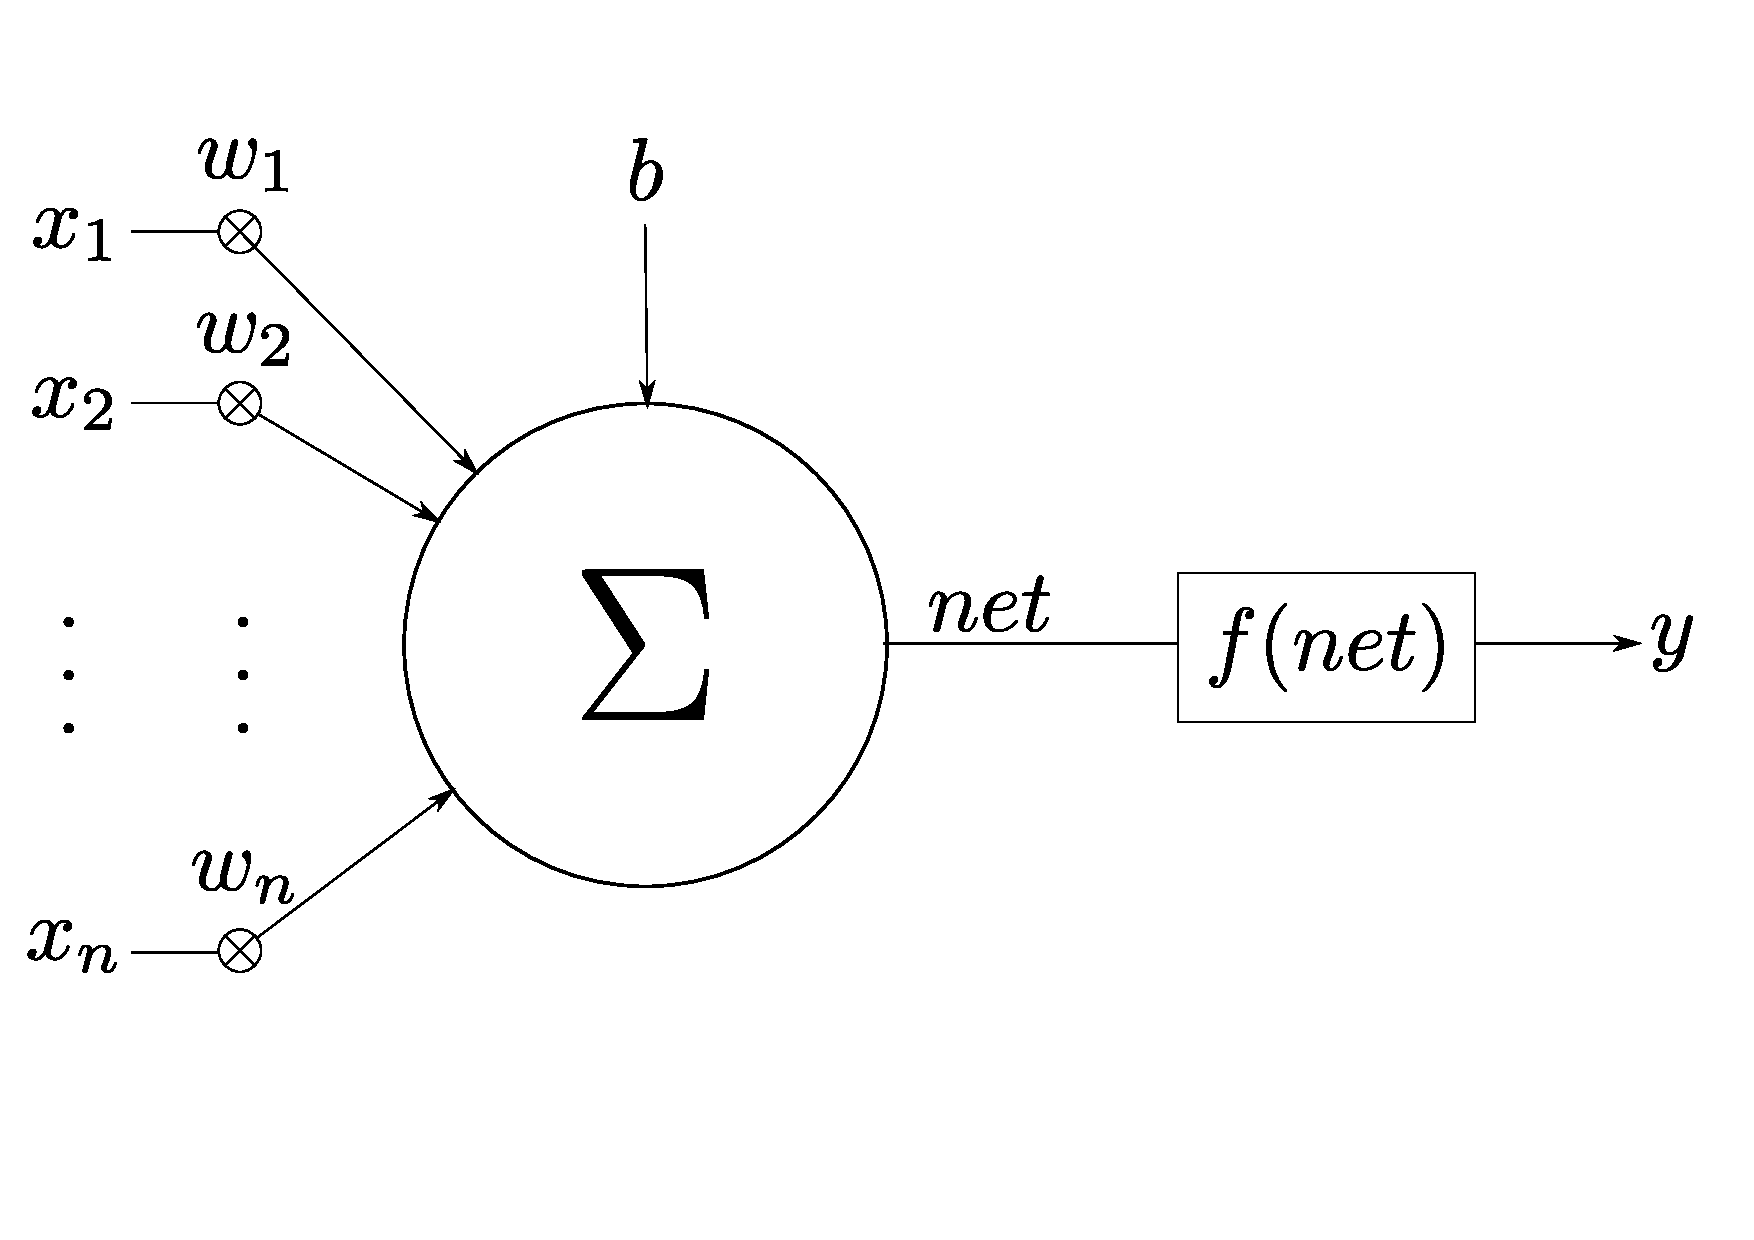
\includegraphics[scale=0.3]{moj_umjetni_neuron.pdf}
	\caption{Umjetni neuron}
	\label{fig:umjetni_neuron}
\end{figure}

Umjetni neuron prima više ulaza $x_1, x_2,...,x_n$ koji tvore ulazni 
vektor $\vec{x}$. Taj ulazni vektor može biti stvarni ulaz ili izlaz iz nekog 
prethodnog neurona. Za svaku vrijednost $x_i$ ulaznog vektora $\vec{x}$
postoji vrijednost $w_i$ koju nazivamo težina (eng. \textit{weight}). To je 
vrijednost koja predstavlja utjecaj ulaza $x_i$ na neuron. Svaki ulaz $x_i$ 
množi se s odgovarajućom težinom $w_i$ što daje umnožak $x_i \cdot w_i$. 
Vrijednosti $w_1, w_2,...,w_n$ tvore vektor težina $\vec{w}$. Još se definira
i vrijednost $b$ koja označava pomak (engl. \textit{bias}). Sve primljene 
vrijednosti se sumiraju prema izrazu \ref{eq: net}.
\begin{equation}
	net = \sum_{i=1}^{n}x_i \cdot w_i + b
	\label{eq: net}
\end{equation}
Izraz \ref{eq: net} može se zapisati u matričnom obliku:
\begin{equation}
	net = \vec{w}^\top \cdot \vec{x} + b
\end{equation}
Pri tome ulazni vektor $\vec{x}$ i vektor težina $\vec{w}$ imaju dimenzije 
N$\times$1, gdje N predstavlja broj ulaza u neuron, dok je pomak $b$ skalar.
Rezultat sumiranja $net$ dalje se predaje kao ulaz prijenosnoj funkciji koja
određuje konačni izlaz $o$ neurona prema izrazu \ref{eq: output}.
\begin{equation}
	y = f(net) = f(\vec{w}^\top \cdot \vec{x} + b)
	\label{eq: output}
\end{equation}
Gdje $f$ predstavlja prijenosnu funkciju.

\subsection{Prijenosne funkcije}
Glavna zadaća prijenosne funkcije je pretvorba ulaznih vrijednosti u izlaznu 
vrijednost. Pri tome se mogu koristiti različite vrste funkcija ovisno o 
arhitekturi mreže. Danas postoji više prijenosnih funkcija koje se češće koriste.
\\\indent
Prva od njih je funkcija skoka i definirana je izrazom \ref{eq:step_fun}.
\begin{equation}
	u(x) = 
	\begin{cases}
		0, \quad x < 0\\
		1, \quad x \geq 0
	\end{cases}
	\label{eq:step_fun}
\end{equation}

Bitno svojstvo ove funkcije je prekid u točki $x=0$, te zbog toga nije 
diferencijabilna u toj točki. Naime, to svojstvo onemogućava korištenje 
algoritama učenja koji se temelje na gradijentu. 
\begin{figure}[htb]
	\centering
	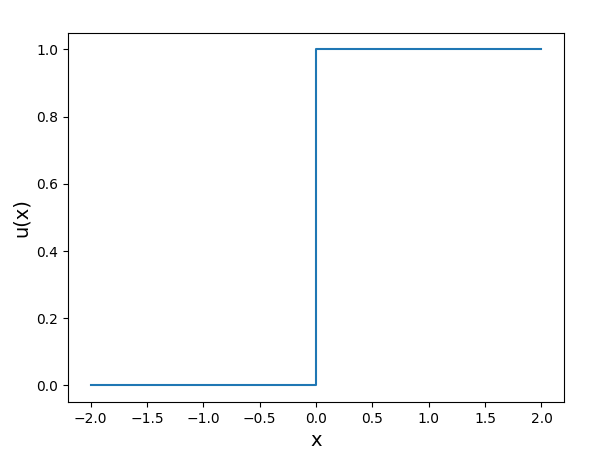
\includegraphics[scale=0.35]{step_fun.png}
	\caption{Funkcija skoka}
	\label{fig:step_fun}
\end{figure}
Izgled funkcije prikazan je na slici 
\ref{fig:step_fun}.
\newpage
Sigmoidalna funkcija ima jako dobra svojstva te se zbog toga često primjenjuje.
Smješta bilo koji realni broj na interval $[0, 1]$. Definirana je izrazom 
\ref{eq:sig}.
\begin{equation}
	\sigma(x)=\frac{1}{1+e^{-x}}
	\label{eq:sig}
\end{equation}
Ova funkcija ima dosta sličnosti s funkcijom skoka. Naime, ako je $x$ neki 
veliki pozitivan broj onda je $e^{-x} \approx 0$, i izlaz iz neurona je blizu
1. S druge strane ako je $x$ neki veliki negativni broj onda $e^{-x} \to 
\infty$, i izlaz iz neurona je blizu 0. To se jako dobro može primijetiti na
grafu funkcije prikazanom na slici \ref{fig:sig_fun}.
\begin{figure}[htb]
	\centering
	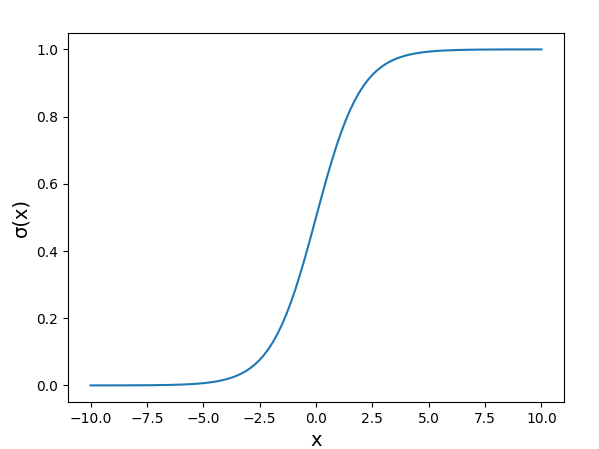
\includegraphics[scale=0.35]{sig_fun.png}
	\caption{Sigmoidalna funckija}
	\label{fig:sig_fun}
\end{figure}

Velika prednost sigmoidalne funkcije u odnosu na funkciju skoka je činjenica da 
je derivabilna, što omogućava korištenje algoritama učenja koji se temelje na 
gradijentu. Derivacija ove funkcije dana je izrazom \ref{eq:dsig}.
\begin{equation}
	\frac{d\sigma(x)}{dx} = \sigma(x)\cdot(1-\sigma(x))
	\label{eq:dsig}
\end{equation}

Na krajevima funkcija jako slabo reagira na promjene i zato će gradijent u tim 
dijelovima imati male vrijednosti. Ako mreža uči pomoću lokalnih gradijenata,
u tom slučaju učenje staje, jer gradijenti ne mogu napraviti značajne promjene.
\\\indent
Funkciju tangens hiperbolni moguće je dobiti izravno iz sigmoidalne funkcije.
Definicija je dana izrazom \ref{eq:tanh}.
\begin{equation}
	tanh(x) = 2\sigma(2x)-1
	\label{eq:tanh}
\end{equation}
Ova prijenosna funkcija smješta bilo koji realni broj na interval $[-1, 1]$.
Prednost je što je derivabilna, ali kao i sigmoidalna funkcija na krajevima jako
slabo reagira na promjene, te ako je vrijednost ulaza u funkciju u tom području, 
učenje staje, što se može vidjeti na grafu funkcije \ref{fig:tanh_fun}. Derivacija 
funkcije dana je izrazom \ref{eq:dtanh}.
\begin{equation}
	\frac{dtanh(x)}{dx} = 1 - tanh^2(x)
	\label{eq:dtanh}
\end{equation}
\begin{figure}[htb]
	\centering
	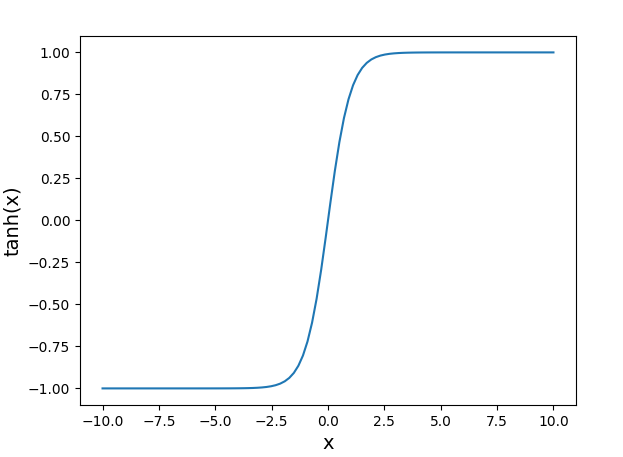
\includegraphics[scale=0.35]{tanh_fun.png}
	\caption{Tangens hiperbolni}
	\label{fig:tanh_fun}
\end{figure}

Zadnjih nekoliko godina sve se češće koristi ReLU (\textit{Recitified Linear 
Unit}) prijenosna funkcija. Određena je izrazom \ref{eg:relu}.
\begin{equation}
	relu(x) = max(0, x)
	\label{eg:relu}
\end{equation}
Ova prijenosna funkcija sve vrijednosti veće od 0 propušta, dok vrijednosti manje 
od 0 uopće ne propušta, što se može vidjeti na grafu funkcije \ref{eg:relu}.
\begin{figure}[htb]
	\centering
	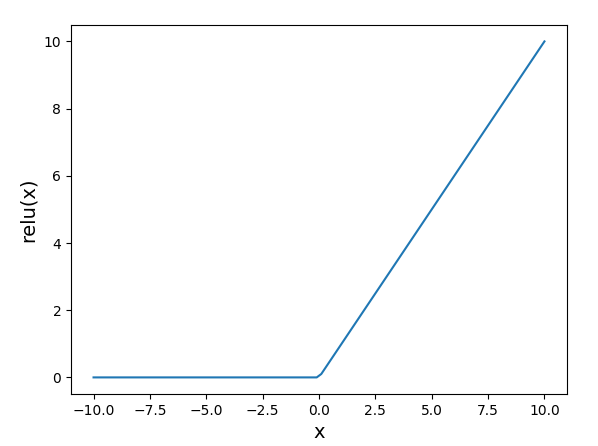
\includegraphics[scale=0.35]{relu_fun.png}
	\caption{ReLU}
	\label{fig:relu_fun}
\end{figure}
\\
Derivacije ove funkcije dana je izrazom \ref{eq:drelu}.
\begin{equation}
	\frac{drelu(x)}{dx} = 
	\begin{cases}
		1, \quad x > 0\\
		0, \quad x \leq 0
	\end{cases}
	\label{eq:drelu}
\end{equation}
Razlog zbog kojeg se sve češće primjenjuje je brzina računanja. Ali i ova 
prijenosna funkcija ima nedostatak. Iz izraza \ref{eq:drelu} se vidi da je 
za sve negativne brojeve derivacija jednaka 0, što predstavlja problem za
algoritme učenja temeljene na gradijentu. Neuron kojemu je suma ulaza, odnosno
$net$ negativan, se zbog toga neće moći prilagođavati.

\section{Arhitektura umjetne neuronske mreže}
Umjetna neuronska mreža sastoji se od više umjetnih neurona koji su međusobno
povezani i grupirani u slojeve. Na slici \ref{fig:ann} je prikazana neuronska
mreža koja ima četiri sloja. Prvi sloj je ulazni i sastoji se od tri neurona,
a zadnji sloj je izlazni i sastoji se od dva neurona. Svaki sloj koji se nalazi
između ulaznog i izlaznog zove se skriveni sloj. 

\begin{figure}[htb]
	\centering
	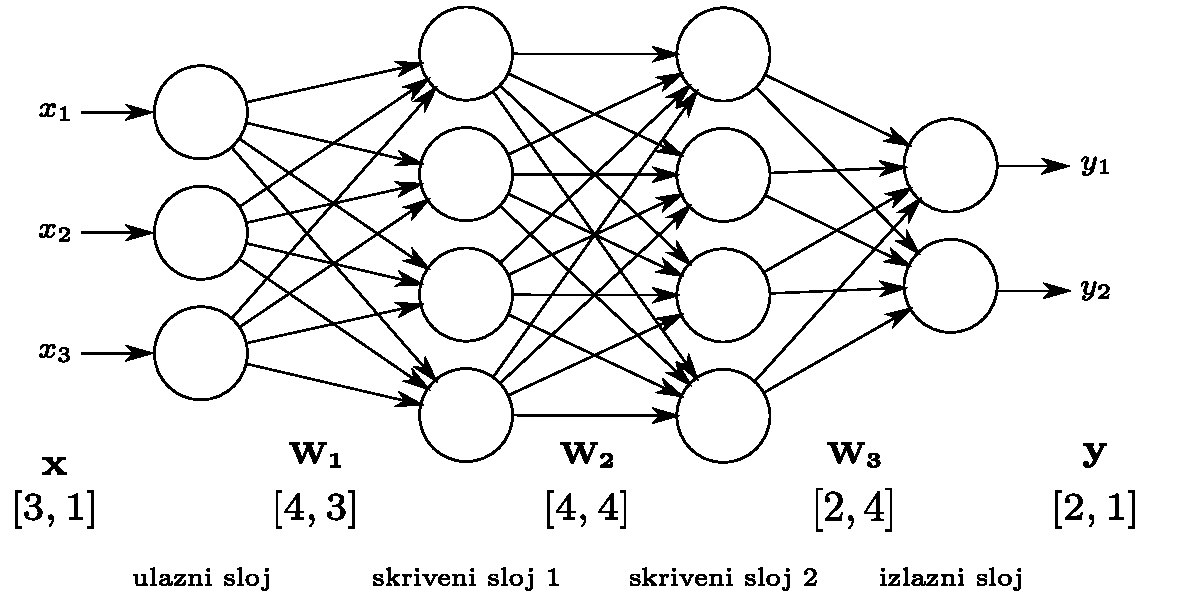
\includegraphics[scale=0.65]{ann.pdf}
	\caption{Umjetna neuronska mreža}
	\label{fig:ann}
\end{figure}

Ovakva mreža zove se još i 
potpuno povezana mreža, jer je izlaz iz svakog neurona u jednom sloju povezan 
sa svim neuronima u idućem sloju. Arhitektura neuronske mreže opisuje
kompoziciju funkcija. Na primjer, mrežu sa slike \ref{fig:ann} možemo opisati 
kompozicijom funkcija $f(\vec{x}) = f^{(3)}(f^{(2)}(f^{(1)}(\vec{x})))$, gdje
$f^{(1)}$ predstavlja prvi skriveni sloj, $f^{(2)}$ drugi skriveni sloj, a
$f^{(3)}$ izlazni sloj. Pri tome su funkcije $f^{(1)}$, $f^{(2)}$, $f^{(3)}$
definirane izrazima: 
\begin{align}
	\vec{h_1} &= f^{(1)}(\vec{x};\vec{W_1}, \vec{b_1}) = g_1(\vec{W_1}\cdot
	\vec{x} +\vec{b_1}) \\
	\vec{h_2} &= f^{(2)}(\vec{h_1};\vec{W_2}, \vec{b_2})= g_2(\vec{W_2}\cdot
	\vec{h_1} +\vec{b_2}) \\
	\vec{y} &= f^{(3)}(\vec{h_2};\vec{W_3}, \vec{b_3}) = g_3(\vec{W_3}\cdot
	\vec{h_2} +\vec{b_3})
\end{align}

Gdje $g_1$, $g_2$ i $g_3$ predstavljaju prijenosne funkcije u pojedinim 
slojevima, a matrice $\vec{W_1}$, $\vec{W_2}$ i $\vec{W_3}$ predstavljaju
matrice težina pojedinih slojeva. Vektori $\vec{b_1}$, $\vec{b_2}$ i $\vec{b_3}$
predstavljaju pomak za svaki sloj.

\section{Učenje umjetne neuronske mreže}
Učenje neuronske mreže je proces nalaženja optimalnih parametara $\pmb{\theta}$,
kako bi neuronska mreža što bolje aproksimirala ciljnu funkciju. Ciljna funkcija
se zaključuje na osnovu uzoraka iz skupa za učenje koji se predočavaju 
neuronskoj mreži. Svaki uzorak je par koji se sastoji od ulaza u mrežu i
željenog izlaza. Ovakav način učenja se zove nadzirano učenje (engl. 
\textit{supervised learning}).
\\\indent
Kako bi odredili koliko dobro mreža aproksimira ciljnu funkciju koristimo
funkciju gubitka. Minimiziranjem funkcije gubitka neuronska mreža se uči.

\subsection{Funkcija gubitka}


\chapter{Konvolucijska neuronska mreža}

\chapter{Zaključak}
Zaključak.

\bibliography{literatura}
\bibliographystyle{fer}
\nocite{Cupic-UNN}
\nocite{Goodfellow-et-al-2016}


\begin{sazetak}
Sažetak na hrvatskom jeziku.

\kljucnerijeci{Ključne riječi, odvojene zarezima.}
\end{sazetak}

% TODO: Navedite naslov na engleskom jeziku.
\engtitle{Title}
\begin{abstract}
Abstract.

\keywords{Keywords.}
\end{abstract}

\end{document}
